\documentclass[aspectratio=169]{beamer}
\usetheme{default}
\usecolortheme{whale}
\setbeamertemplate{navigation symbols}{}
\setbeamertemplate{footline}{}
\setbeamertemplate{headline}{}
\setbeamerfont{title}{size=\Large,series=\bfseries}
\setbeamerfont{frametitle}{size=\Large,series=\bfseries}

\usepackage{amsmath,amssymb}
\usepackage{graphicx}
\usepackage{tikz}
\usepackage{xcolor}
\usetikzlibrary{shapes,arrows.meta,positioning,fit,backgrounds,decorations.pathreplacing}

\definecolor{ok}{HTML}{2ca02c}
\definecolor{bad}{HTML}{d62728}
\definecolor{sig}{HTML}{1f77b4}
\definecolor{smx}{HTML}{ff7f0e}

\title{When models are confidently wrong}
\subtitle{Catching receipt-total errors by checking the math}
\author{ASYU 2026}
\date{}

\begin{document}

% ==========================================================
\frame{\titlepage}

% ==========================================================
\begin{frame}{}
\vfill
\begin{center}
{\Huge A model reads a receipt.}\\[0.6em]
{\Huge It says the total is \textbf{\textcolor{sig}{\$58.40}}.}\\[1.2em]
{\Large Is it right?}
\end{center}
\vfill
\begin{tikzpicture}[remember picture,overlay]
\node[anchor=south east] at (current page.south east)
  [xshift=-1cm,yshift=1cm]
  {\begin{tikzpicture}[scale=0.55]
    \draw[fill=white,thick] (0,0) rectangle (4,6);
    \draw (0.3,5.5) -- (3.7,5.5);
    \node at (2,5.7) {\small\bfseries RECEIPT};
    \node[anchor=west] at (0.3,4.8) {\small Coffee \hfill \$3.20};
    \node[anchor=west] at (0.3,4.3) {\small Sandwich \hfill \$8.50};
    \node[anchor=west] at (0.3,3.8) {\small Salad \hfill \$6.00};
    \node[anchor=west] at (0.3,3.3) {\small ...};
    \draw (0.3,2.7) -- (3.7,2.7);
    \node[anchor=west] at (0.3,2.2) {\small Subtotal \hfill \$52.40};
    \node[anchor=west] at (0.3,1.7) {\small Tax \hfill \$6.00};
    \draw[thick] (0.3,1.2) -- (3.7,1.2);
    \node[anchor=west] at (0.3,0.7) {\small\bfseries TOTAL \hfill \textbf{?}};
  \end{tikzpicture}};
\end{tikzpicture}
\end{frame}

% ==========================================================
\begin{frame}{}
\begin{center}
{\Large The usual way: \emph{ask the model how confident it is.}}
\end{center}
\vspace{1em}
\begin{center}
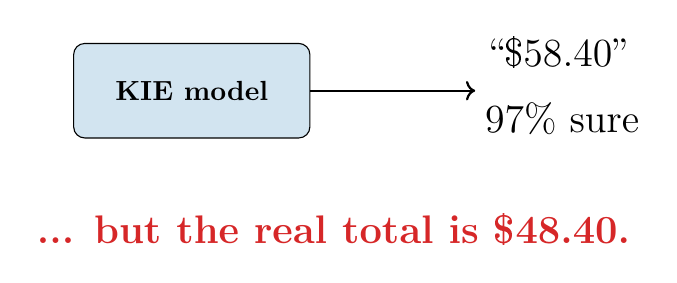
\begin{tikzpicture}[scale=1.2]
\node[draw,rounded corners,fill=sig!20,minimum width=3cm,minimum height=1.2cm] (m) at (0,0) {\textbf{KIE model}};
\node[anchor=west] at (3,0.4) {\Large ``\$58.40''};
\node[anchor=west] at (3,-0.3) {\Large 97\% sure};
\draw[->,thick] (m.east) -- (3,0);
\node[anchor=north] at (1.5,-1.2) [text=bad] {\Large\bfseries ... but the real total is \$48.40.};
\end{tikzpicture}
\end{center}
\vspace{1em}
\begin{center}
\textbf{\textcolor{bad}{The model can be confidently wrong.}}\\
Softmax is the model's opinion of \emph{itself}.
\end{center}
\end{frame}

% ==========================================================
\begin{frame}{}
\vfill
\begin{center}
{\Large \textbf{What if we just \emph{check the math?}}}\\[1em]
{\large The receipt has all the numbers.}\\
{\large Do any of them add up to the prediction?}
\end{center}
\vfill
\end{frame}

% ==========================================================
\begin{frame}{}
\begin{center}
{\large Our gate: $\sigma$}
\end{center}
\vspace{0.5em}
\begin{center}
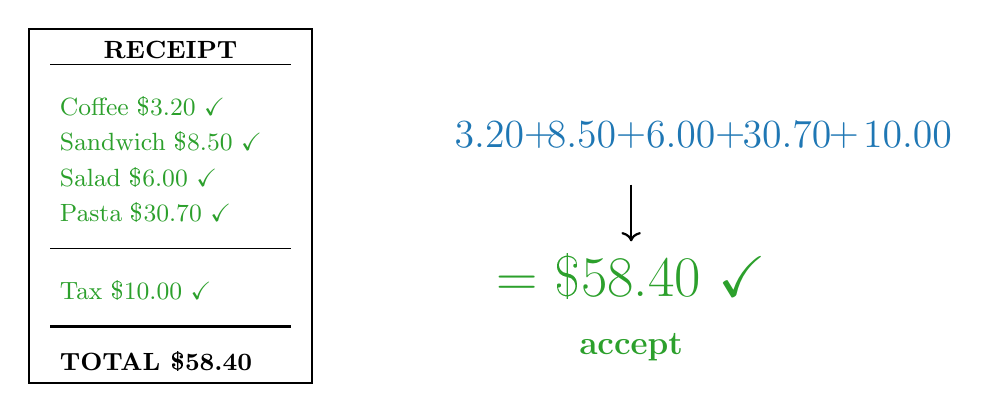
\begin{tikzpicture}[scale=0.9]
\draw[fill=white,thick] (0,0) rectangle (4,5);
\draw (0.3,4.5) -- (3.7,4.5);
\node at (2,4.7) {\small\bfseries RECEIPT};
\node[anchor=west,text=ok] at (0.3,3.9) {\small Coffee \hfill \$3.20 \checkmark};
\node[anchor=west,text=ok] at (0.3,3.4) {\small Sandwich \hfill \$8.50 \checkmark};
\node[anchor=west,text=ok] at (0.3,2.9) {\small Salad \hfill \$6.00 \checkmark};
\node[anchor=west,text=ok] at (0.3,2.4) {\small Pasta \hfill \$30.70 \checkmark};
\draw (0.3,1.9) -- (3.7,1.9);
\node[anchor=west,text=ok] at (0.3,1.3) {\small Tax \hfill \$10.00 \checkmark};
\draw[thick] (0.3,0.8) -- (3.7,0.8);
\node[anchor=west] at (0.3,0.3) {\small\bfseries TOTAL \hfill \$58.40};

\node at (6.5,3.5) [text=sig,font=\Large] {3.20};
\node at (7.2,3.5) [text=sig,font=\Large] {+};
\node at (7.8,3.5) [text=sig,font=\Large] {8.50};
\node at (8.5,3.5) [text=sig,font=\Large] {+};
\node at (9.2,3.5) [text=sig,font=\Large] {6.00};
\node at (9.9,3.5) [text=sig,font=\Large] {+};
\node at (10.7,3.5) [text=sig,font=\Large] {30.70};
\node at (11.5,3.5) [text=sig,font=\Large] {+};
\node at (12.4,3.5) [text=sig,font=\Large] {10.00};

\draw[->,thick] (8.5,2.8) -- (8.5,2.0);
\node at (8.5,1.5) [text=ok,font=\huge] {= \$58.40 \checkmark};
\node at (8.5,0.5) [text=ok,font=\large] {\textbf{accept}};
\end{tikzpicture}
\end{center}
\end{frame}

% ==========================================================
\begin{frame}{}
\vfill
\begin{center}
{\large \textbf{Two signals that miss \emph{different} receipts}}
\end{center}
\vspace{1em}
\begin{center}
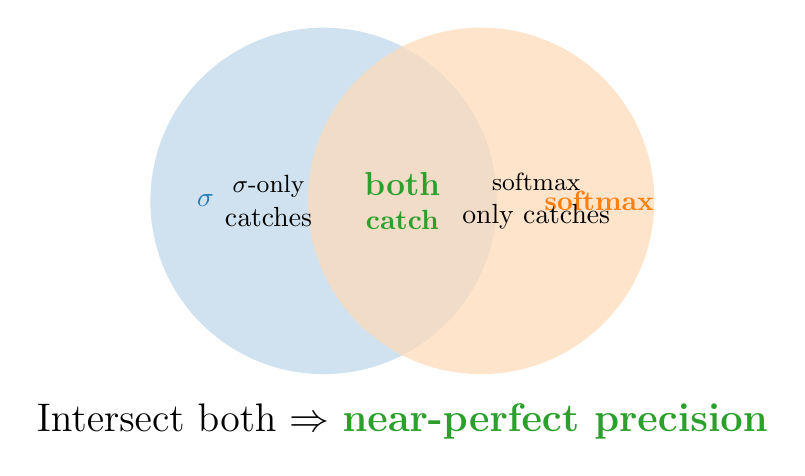
\begin{tikzpicture}[scale=1.0]
\fill[sig!30,opacity=0.7] (-1,0) circle (2.2);
\fill[smx!30,opacity=0.7] (1,0) circle (2.2);
\node at (-2.5,0) [text=sig,font=\bfseries] {$\sigma$};
\node at (2.5,0) [text=smx,font=\bfseries] {softmax};

\node[align=center] at (-1.7,0) {\small $\sigma$-only\\catches};
\node[align=center,text=ok,font=\bfseries] at (0,0) {\large both\\catch};
\node[align=center] at (1.7,0) {\small softmax\\only catches};

\node at (0,-2.8) [font=\Large] {Intersect both $\Rightarrow$ \textbf{\textcolor{ok}{near-perfect precision}}};
\end{tikzpicture}
\end{center}
\vfill
\end{frame}

% ==========================================================
\begin{frame}{}
\vfill
\begin{center}
{\huge On 919 real receipts:}\\[1.5em]
{\Huge\bfseries\textcolor{ok}{precision = 0.988}}\\[0.5em]
{\large (160 correct out of 162 accepts)}\\[2em]
{\Large Wilson 95\% lower bound: \textbf{0.956}}\\[1em]
{\large Both single signals alone: below 0.92}
\end{center}
\vfill
\end{frame}

% ==========================================================
\begin{frame}{}
\begin{center}
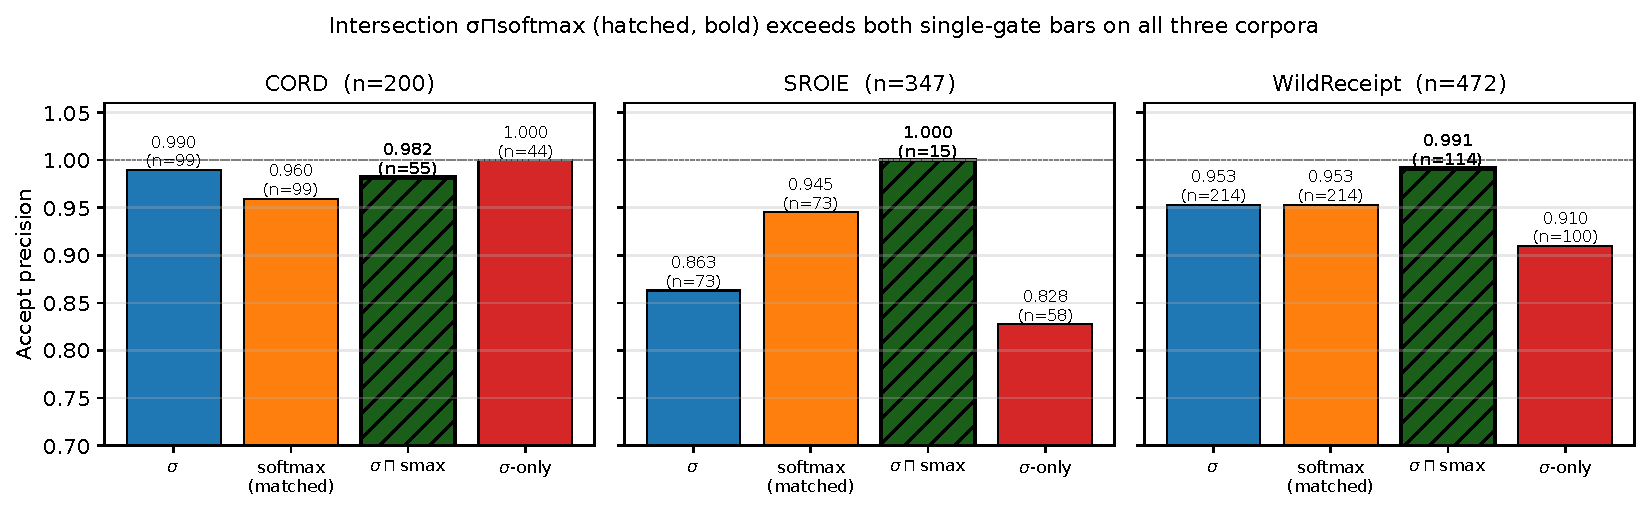
\includegraphics[width=0.95\linewidth]{figures/fig_overview.pdf}
\end{center}
\begin{center}
\large \textbf{Three datasets. Two model architectures. Same answer.}
\end{center}
\end{frame}

% ==========================================================
\begin{frame}{}
\begin{center}
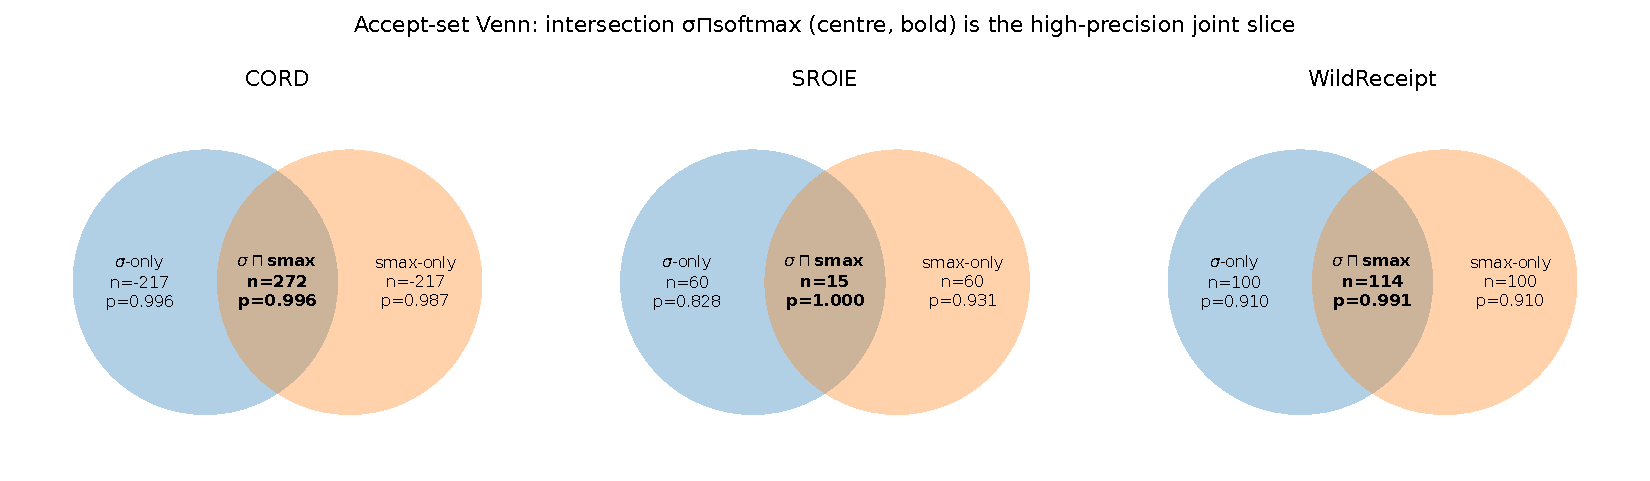
\includegraphics[width=0.85\linewidth]{figures/fig_accept_venn.pdf}
\end{center}
\begin{center}
\large The \emph{middle} of each Venn is the joint accept slice. Always more precise.
\end{center}
\end{frame}

% ==========================================================
\begin{frame}{}
\vfill
\begin{center}
{\Large \textbf{Striking case: WildReceipt}}\\[1em]
\begin{tikzpicture}[scale=1.1]
\draw[fill=sig!30] (0,0) rectangle (2,3.2);
\node at (1,3.5) {$\sigma$ alone};
\node at (1,-0.4) {\Large \textbf{0.953}};

\draw[fill=smx!30] (3,0) rectangle (5,3.2);
\node at (4,3.5) {softmax alone};
\node at (4,-0.4) {\Large \textbf{0.953}};

\draw[fill=ok!50,pattern=north east lines,pattern color=ok] (6,0) rectangle (8,3.32);
\node at (7,3.5) {intersection};
\node at (7,-0.4) {\Large \textbf{\textcolor{ok}{0.991}}};
\end{tikzpicture}\\[1.5em]
{\large The two signals are \emph{equally accurate alone}.}\\[0.5em]
{\large But they fail on \emph{different} receipts.}\\[0.5em]
{\large Intersection still wins.}
\end{center}
\vfill
\end{frame}

% ==========================================================
\begin{frame}{}
\vfill
\begin{center}
{\Large \textbf{How expensive?}}\\[2em]
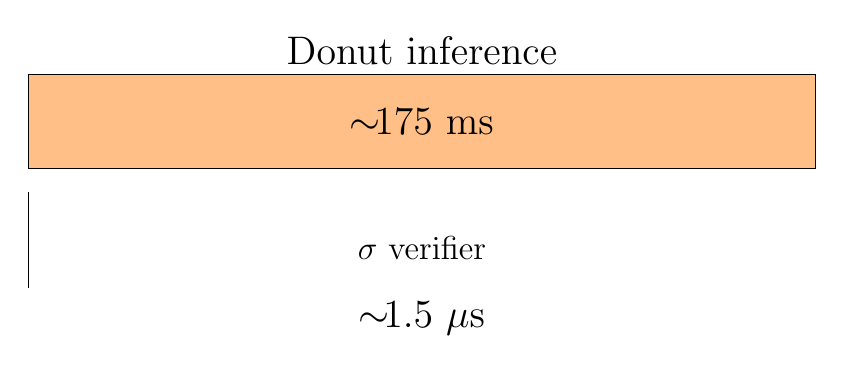
\begin{tikzpicture}
\draw[fill=smx!50] (0,0) rectangle (10,1.2);
\node at (5,1.5) {\Large Donut inference};
\node at (5,0.6) {\Large $\sim$\!175 ms};
\draw[fill=sig!50] (0,-1.5) rectangle (0.0016,-0.3);
\node at (5,-1) {\large $\sigma$ verifier};
\node at (5,-1.9) {\Large $\sim$\!1.5 $\mu$s};
\end{tikzpicture}\\[1em]
{\Large $\sigma$ adds \textbf{\textcolor{ok}{0.0016\%}} to total latency.}\\[0.5em]
{\large Effectively free.}
\end{center}
\vfill
\end{frame}

% ==========================================================
\begin{frame}{}
\vfill
\begin{center}
{\Huge \textbf{Take-home}}\\[2em]
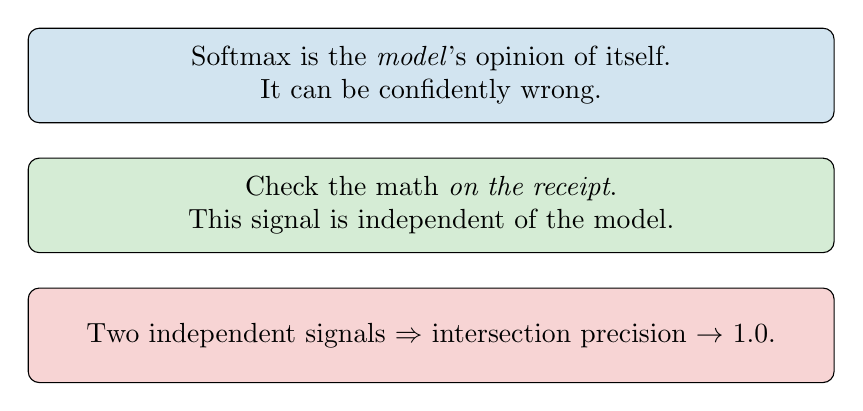
\begin{tikzpicture}[scale=1.1]
\node[draw,rounded corners,fill=sig!20,text width=10cm,align=center,minimum height=1.2cm] at (0,1.5)
  {Softmax is the \emph{model}'s opinion of itself.\\It can be confidently wrong.};
\node[draw,rounded corners,fill=ok!20,text width=10cm,align=center,minimum height=1.2cm] at (0,0)
  {Check the math \emph{on the receipt}.\\This signal is independent of the model.};
\node[draw,rounded corners,fill=bad!20,text width=10cm,align=center,minimum height=1.2cm] at (0,-1.5)
  {Two independent signals $\Rightarrow$ intersection precision $\to$ 1.0.};
\end{tikzpicture}
\end{center}
\vfill
\begin{center}\large \emph{Thank you. Questions?}\end{center}
\end{frame}

\end{document}
